%\documentclass[0-main.tex]{subfiles}
%\begin{document}

\section{Experiments}\label{sec:exp}
We evaluate \hirl in a series of standard RL benchmarks. Each experimental scenario follows a similar pattern: (1) we generate demonstration trajectories of the task, (2) apply \hirl to learn a reward function, (3) and compare how quickly a Q-learning RL agent converges to a solution with rewards learned with \hirl compared to other techniques.
In principle, the IRL problem (which learns rewards) is orthogonal to the problem of policy search (turning rewards into policies).
One could also use the same reward functions in optimal control frameworks such as iLQR, and we hope to explore this in further detail in future work. 

\subsection{Metrics}
For efficacy, we measure the max expected reward achieved by the agent (i.e., maximum over the entire learning epoch where we evaluate the policy after each episode and take the expected reward). For convergence rate, we measure the Area Under Curve of the learning curve (i.e., cumulative expected reward accrued over the entire learning epoch).
We compare against against IRL and RL directly on a default ``natural" reward function; which was defined as binary success or failure in discrete tasks and the squared distance to rewards in the continuous tasks.
We also include a comparison with direct policy learning from the demonstrations with a multi-class SVM\footnote{\url{http://scikit-learn.org/stable/modules/multiclass.html}} where applicable.

\subsection{2D Discrete Motion Planning}\label{exp:2dmp}
We modified a variant of one of the canonical RL domains, GridWorld, to illustrate how \hirl addresses problems of sequentiality (Figure \ref{exp:gweasy1}). 
This experiment intuitively illustrates the challenge of sequential rewards in RL.
We constructed a grid world with two goal states denoted by ``0'' and ``1'' separated by a narrow passage.
The agent can only receive the reward at ``1'' if it has previously reached ``0".
In the natural $(x,y)$ state-space, the agent does not learn a correct stationary policy since at some states the optimal action depends on knowing whether ``0'' has been reached.
We visualize the Q function of applying RL without state-space augmentation and we find that it predictably struggles in the narrow passage.

In the next figure, we show that augmenting the state-space with sub-task progress learned by \hirl from 5 demonstrations results in a Q function that reflects the sequential nature of the task.
For this task, we find that with \hirl, we can successfully learn a policy that has the desired sequential behavior.
Figure \ref{exp:gweasy1} also shows that \hirl converges faster than solving independent RL problems (K-RL).

\begin{figure}[t]
\centering
 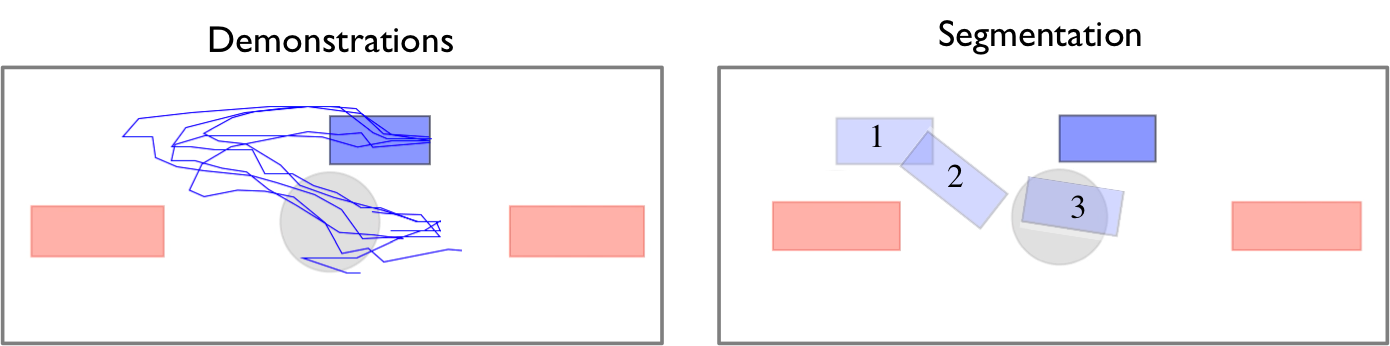
\includegraphics[width=\columnwidth]{exp/rc-car-segmentation.png}
 \caption{This plot illustrates the 5 demonstration trajectories for the parallel parking task, and the sub-goals learned by \hirl. Section \ref{exp:pp} describes the details of the experimental setup and the task. \label{exp:rcsegmentation}}
\end{figure}

\begin{figure}[t]
\centering
 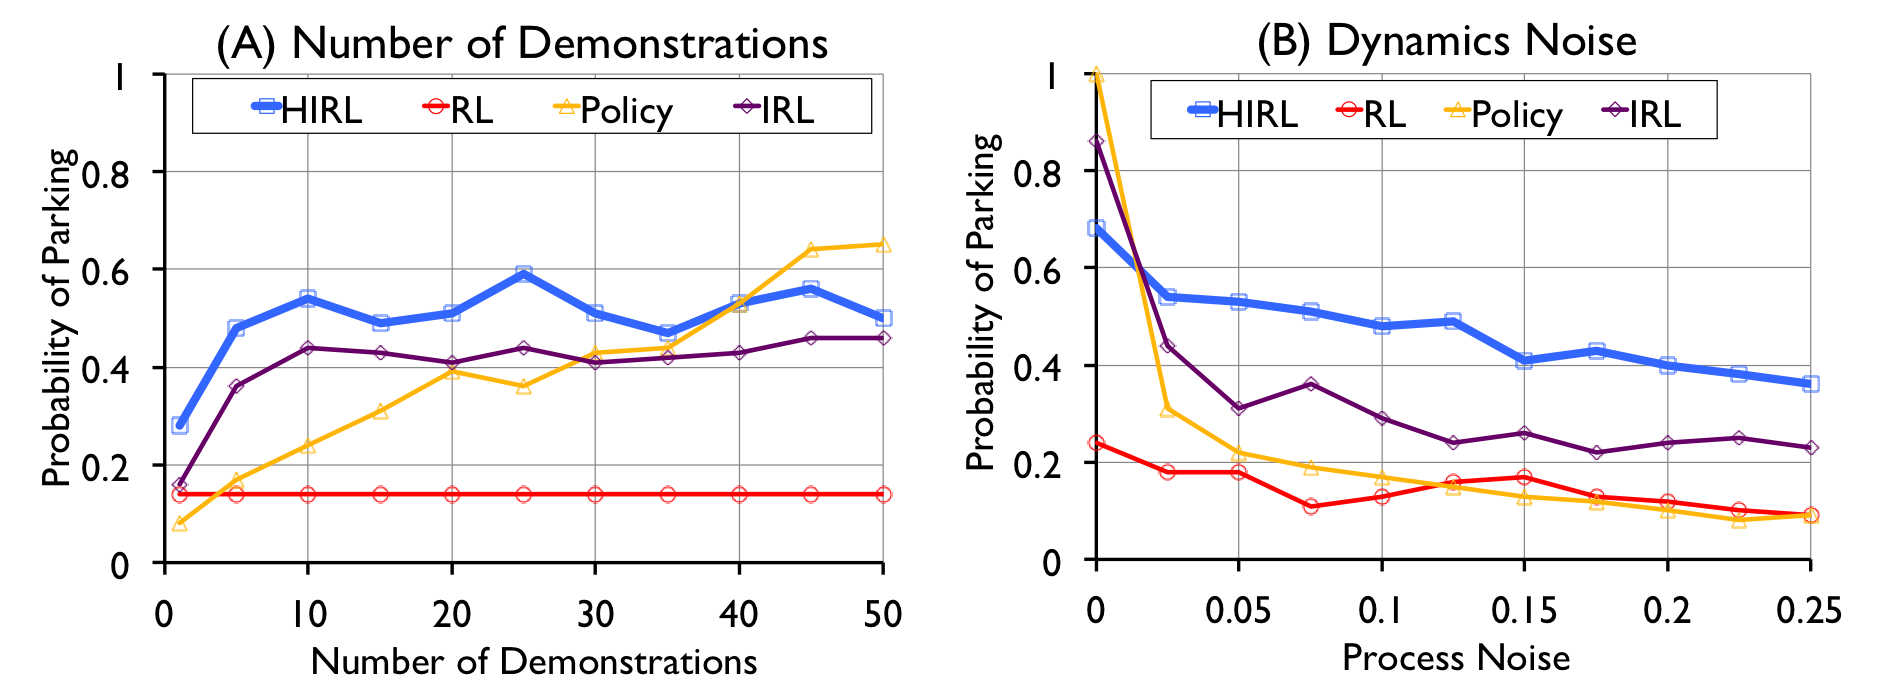
\includegraphics[width=\columnwidth]{exp/rc-car-segmentation-2ab.png}
 \caption{For a fixed number of RL episodes, we measure the success of the policies learned for each of the alternatives (Section \ref{exp:ppr}). [A] We vary the number of demonstrations provided to the different techniques and measure the success probability of the policies learned. \hirl has a higher success rate than the alternatives for a small number of demonstrations. [B] When there is no process noise, directly applying an open-loop policy works. However, we find that \hirl is more robust than the alternatives.  \label{exp:rcsegmentation-res2}}
\end{figure}

\begin{figure}[t]
\centering
 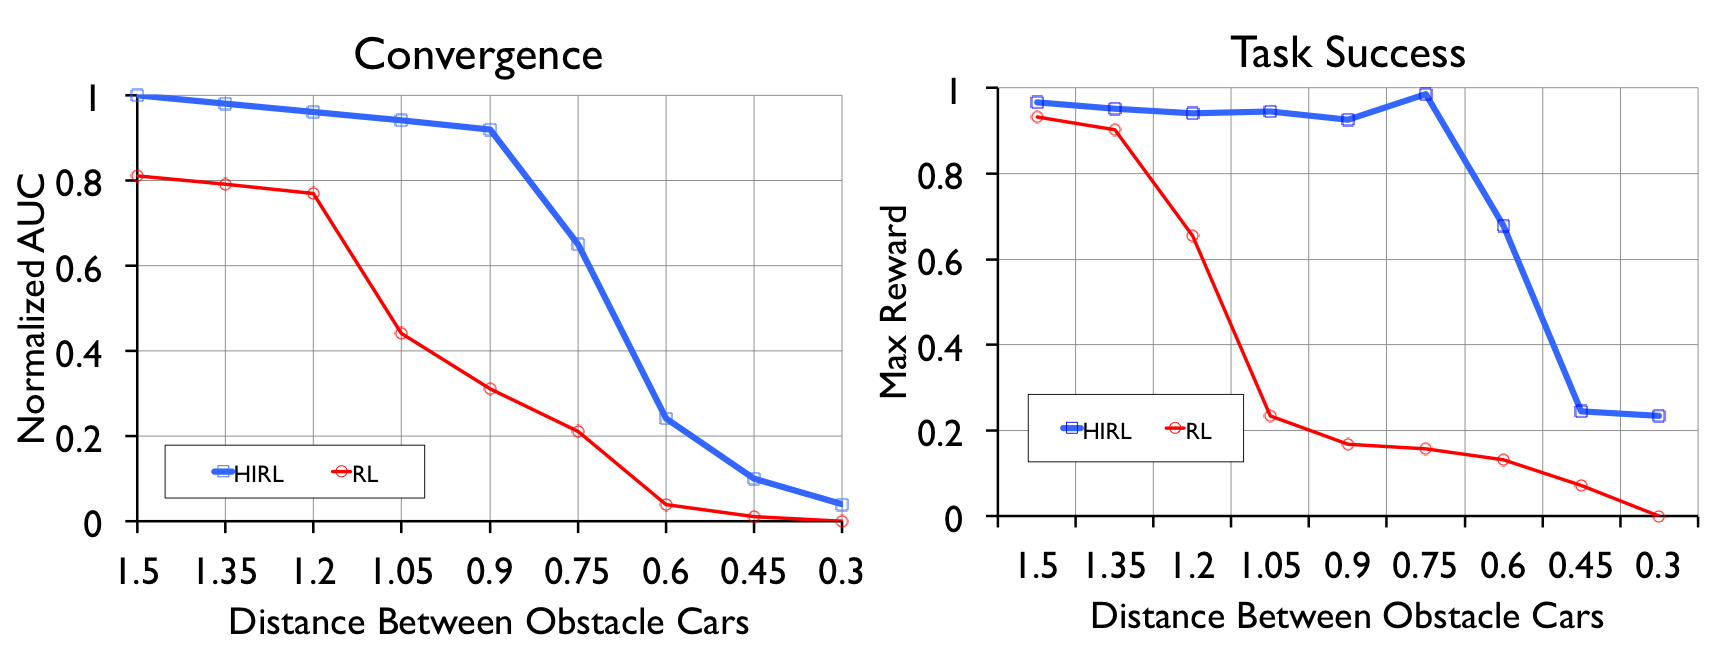
\includegraphics[width=\columnwidth]{exp/rc-env1.png}
 \caption{For a fixed number of RL episodes and 5 demonstrations, we plot the performance of \hirl as a function of the distance between the obstacle parked cars (Section \ref{exp:ppd}). 
 When the distance is large (the task is easier) the gap between \hirl and RL is smaller, however, as the task becomes harder the subgoals are more valuable. \label{exp:rcenv}}
\end{figure}

\begin{figure}[t]
\centering
 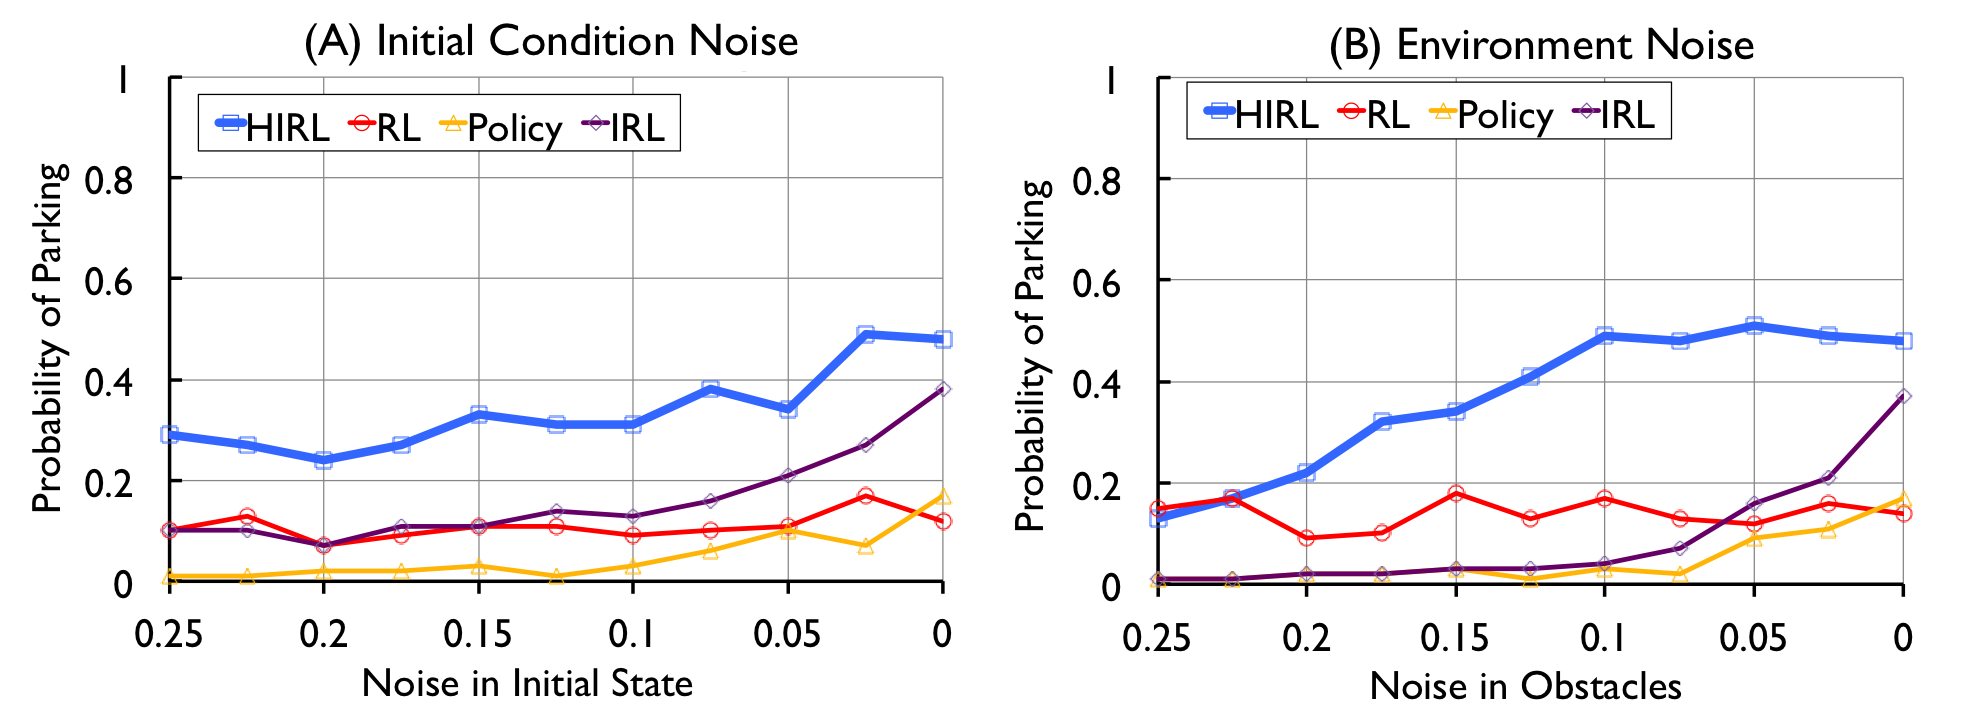
\includegraphics[width=\columnwidth]{exp/rc-env2.png}
 \caption{We collected 5 demonstrations in one environment and applied \hirl, the baseline, and policy learning, and measured the success rate of the learned policies for a fixed number of RL iterations. We evaluated these policies in a randomly perturbed  environment (Section \ref{exp:pper}). Noise is listed in terms of $\sigma$.\label{exp:rcenv2}}
\end{figure}

\iffalse
\begin{figure*}[t]
\centering
 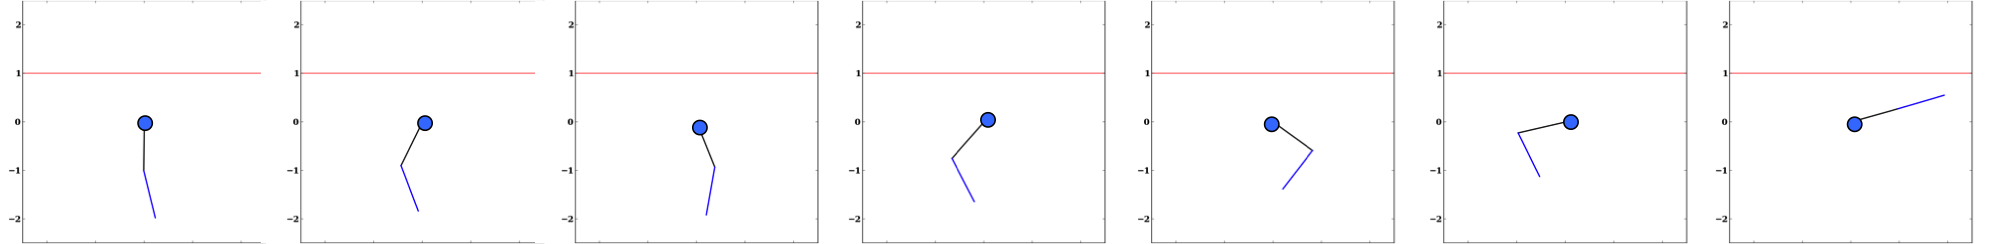
\includegraphics[width=\textwidth]{exp/segmentation-acrobot-segments.png}
 \caption{We apply \hirl to segment 5 demonstrations of Acrobot trajectories. We visualize the segments, and we find that these provide sub-goals for the agent to reach the threshold.\label{exp:acroseg} \todo{this figure isnt as useful as we would like it to be}}
\end{figure*}
\fi

\subsection{Parallel Parking}\label{exp:pp}
We constructed a parallel parking scenario with an agent with non-holonomic dynamics and two obstacles. The agent can control its speed ($\|\dot{x}\|+\|\dot{y}\|$) and heading, and observe its x position, y position, orientation, and speed in a global coordinate frame.
If the agent parks between the obstacles, i.e., 0 velocity within a $15^\circ$ tolerance, the task is a success and the agent receives a reward of $1$. 
The agent's dynamics are noisy and with probability 0.1 will randomly add or subtract $5^\circ$ degrees from the steering angle.
If the agent collides with one of the obstacle or does not park in 200 timesteps the episode ends.
Next, we made the  Parallel Parking domain a little harder. We hid the velocity state from the agent, so the agent only sees $(x,y,\theta)$. As before, if the agent collides with one of the obstacle or does not park in 200 timesteps the episode ends.
We call this domain Parallel Parking-PO.

We collected 5 demonstrations and applied \hirl to learn the segments.
Figure \ref{exp:rcsegmentation} illustrates the demonstrations and the learned segments. There are two intermediate goals corresponding to positioning the car and orienting the car correctly before reversing.

\subsubsection{Convergence}\label{exp:ppc} In the first experiment, we use these learned segments to construct rewards in both the fully observed and partially observed problems (Figure \ref{exp:rcsegmentation-res}). 
In the fully observed problem, compared to IRL, \hirl converges to a policy with a 60\% success rate with about 3x less time-steps of exploration.
After 1250 episodes, the policy learned with \hirl has an 93\% success rate in comparison to a 60\% success rate for the baseline.
Also, for the same number of demonstrations, directly learning a policy gives a success rate of 17\%.

In the partial observation problem, there is no longer a stationary policy that can achieve the reward.
The learned segments help disambiguate dependence on history.
After 2000 episodes, the policy learned with \hirl has an 86\% success rate in comparison to a <10\% success rate for the baseline and the policy learning.

\subsubsection{Demonstrations and Robustness to Process Noise}\label{exp:ppr} Of course, the direct policy learning approach will work well if there is no stochasticity in the environment (i.e., open-loop control).
We evaluate these tradeoffs in the next experiment (Figure \ref{exp:rcsegmentation-res2}). 
If there is no process noise, the policy learning approach works perfectly for a fixed 5 demonstrations.
However even after adding a small amount of process noise, we find that its accuracy immediately drops.
Furthermore, we find that to achieve the same level of accuracy as \hirl after 250 episodes of exploration, need 40 demonstrations for the policy learning approach.

\subsubsection{Task Difficulty}\label{exp:ppd} Next, we explored the benefits of segmentation as a function of the hardness of the task.
We varied the distance between the obstacle cars and measured the performance of \hirl, where a smaller distance would make the task harder.
In comparison to the baseline, we found that segmentation is most beneficial when the task is harder (Figure \ref{exp:rcenv}). 

\begin{figure}[t]
\centering
 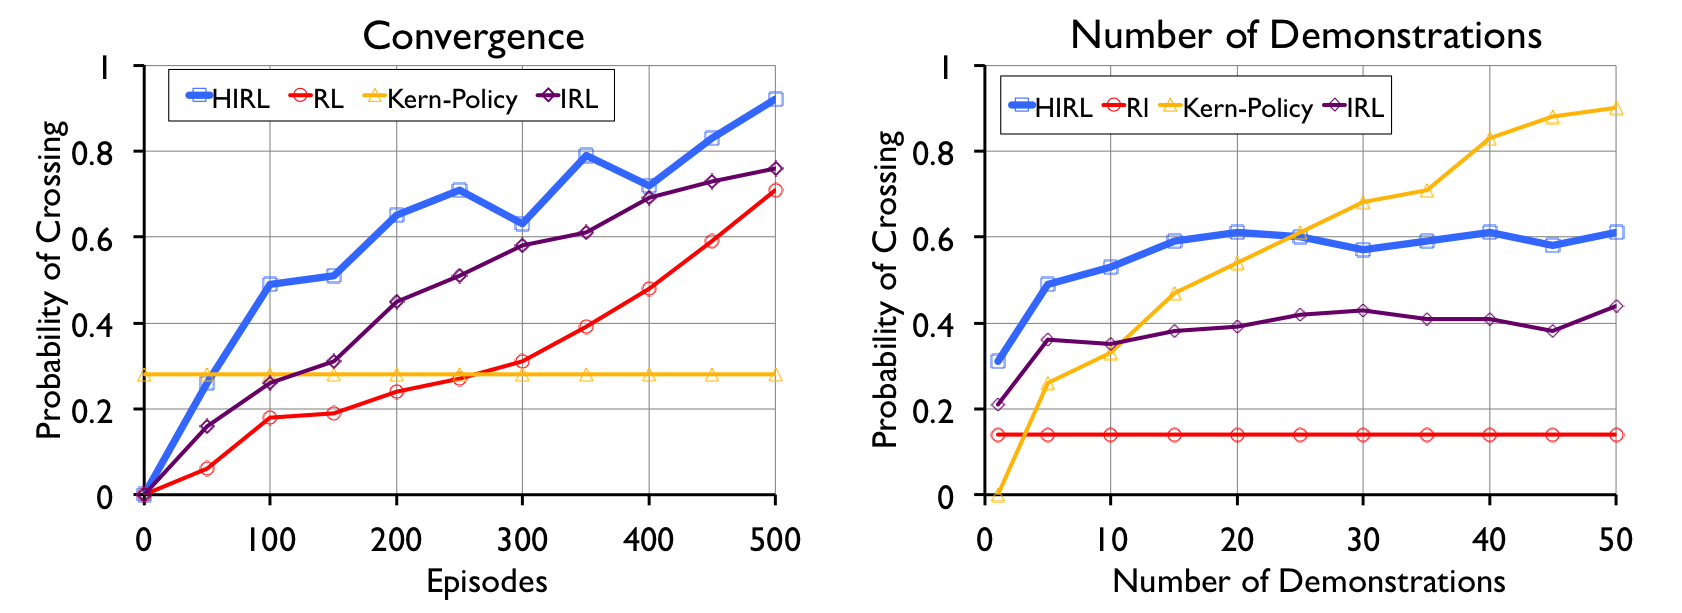
\includegraphics[width=\columnwidth]{exp/acrobot-segmentation-1ab.png}
 \caption{We measured the convergence of rewards constructed with \hirl and the alternatives (Section \ref{exp:acrobot}).
 [A] the success rate of the learned policy for 5 demonstrations, and varying the number of RL episodes. 
 [B] the success rate of the learned policy for a fixed number of episodes and varying the number of demonstrations.  \label{exp:acsegmentation-res2}}
\end{figure}

\subsubsection{Robustness to Environment Noise}\label{exp:pper} Finally, we explored the robustness of the learned policies to changes in the environment and starting position (Figure \ref{exp:rcenv2}).
We collected 5 demonstrations in one environment and applied \hirl, the baseline, and policy learning.
Then, we randomly perturbed the environment and evaluated the success rate of each policy.
We found that the policies learned with segmentation were very robust to noise in the initial state (i.e., the starting pose of the car).
On the other hand, the directly learned policies are not as robust to such noise.
While the actions at every state may change, the sub-goals stay the same.
We also found that the policies learned with segmentation were robust to noise in the obstacle car pose up to a point.

\subsection{Acrobot}\label{exp:acrobot}
This domain consists of a two-link pendulum with gravity and with torque controls on the joint. The dynamics are noisy and there are limits on the applied torque. The agent has 1000 timesteps to raise the arm above horizontal ($y=1$ in the images). If the task is a success and the agent receives a reward of $1$. 
Thus, the expected reward is equivalent to the probability that the current policy will successfully raise the arm above horizontal.
We generated $N=5$ demonstrations for the Acrobot task and applied segmentation. 
%We visualize the learned segments in Figure \ref{exp:acroseg}, which can be seen to qualitatively describe a successful path.
In Figure \ref{exp:acsegmentation-res2}, we plot the convergence of the all of the approaches.
We include a comparison between a Linear Multiclass SVM and a Kernelized Multiclass SVM for the policy learning alternative.
As before, we find that \hirl requires less demonstrations to converge to a more reliable policy.
\hirl converges 2.5x faster to a policy with a success rate of 60\%, and the direct policy learning outperforms \hirl for a fixed 100000 steps only after 25 demonstrations.

\begin{figure*}[t]
\centering
 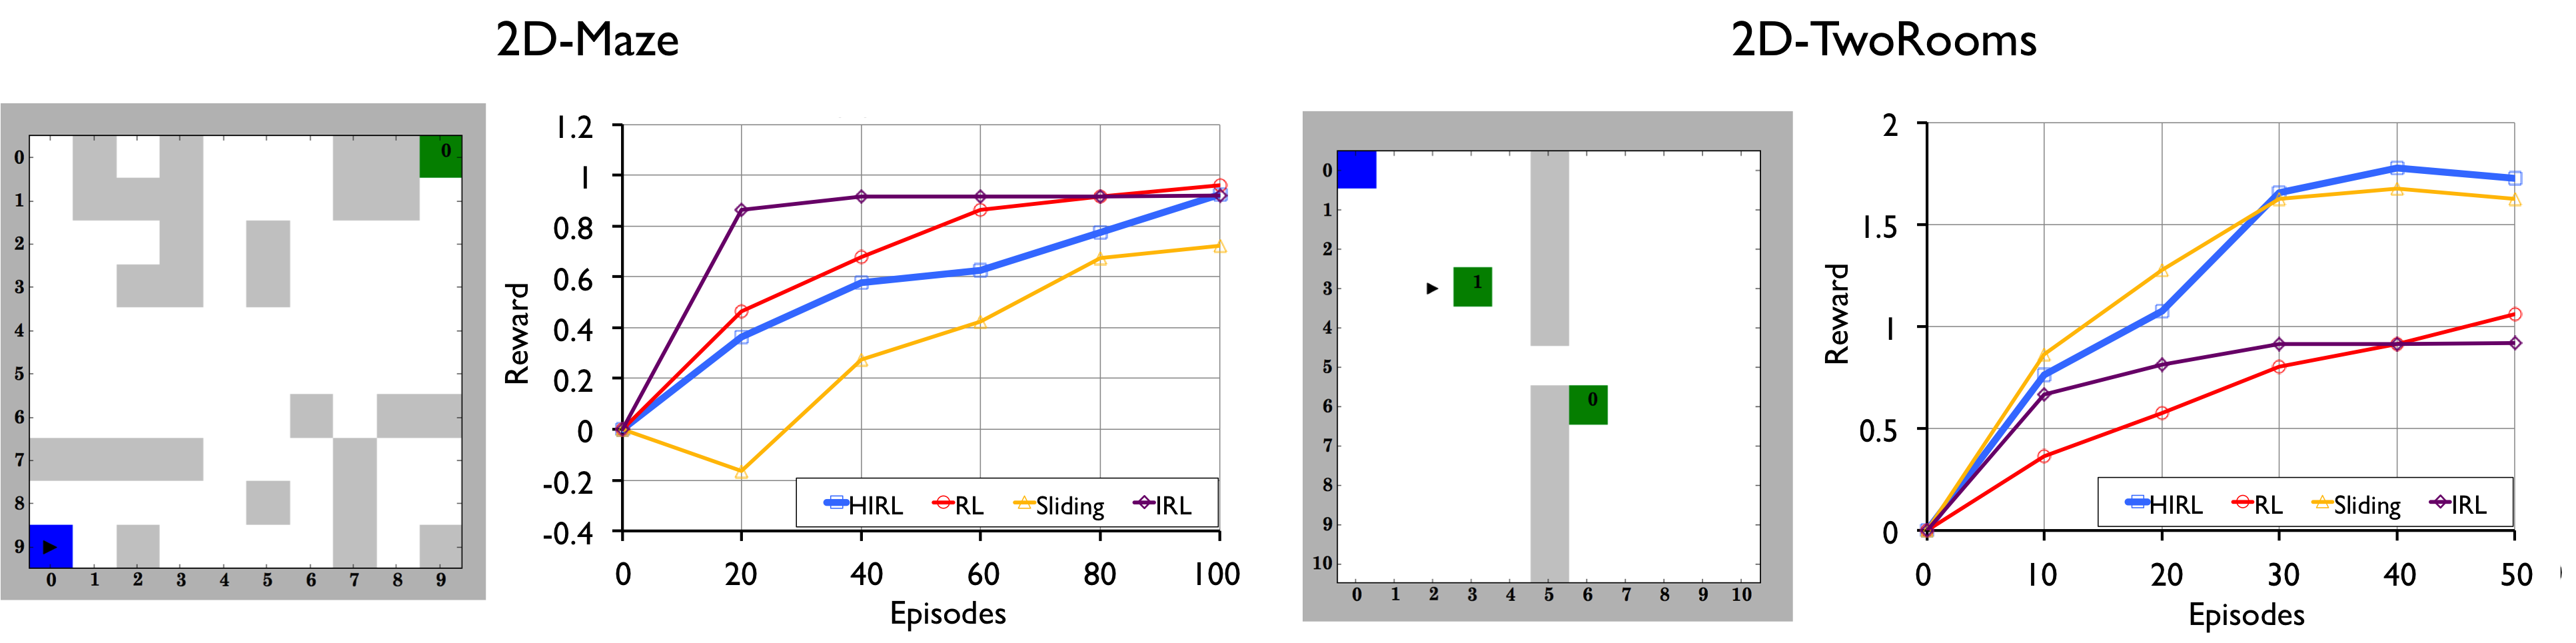
\includegraphics[width=\textwidth]{exp/counter-examples.png}
 \caption{We summarize the results on two further domains (Section \ref{exp:further}). In the Maze domain, an agent plans a path to a single goal. We find that rewards constructed with IRL converge the fastest on this task. In the Two-Rooms domain, we find that alternative state-augmentation techniques ensure convergence, i.e., we can use a sliding window of states. It may not be possible to hard-code such augmentations in all cases, and \hirl provides a general framework to learn subtasks and augment the state-space with the appropriate variables.}
 \label{exp:gw2}
\end{figure*}

\subsection{Further Experiments}\label{exp:further}
Next, we highlight two additional scenarios that we constructed to evaluate \hirl.

\subsubsection{2D-Maze} In this domain, the agent solves a 2D Maze in a 11x10 grid (Figure \ref{exp:gw2}). There is no noise in the dynamics and there is a unique free path from start to end.
The MW domain was constructed to illustrate that over-segmenting a unique solution path can slow down convergence.
There is a single unique path that solves the maze, and this path is essentially revealed with IRL. Adding segments in addition to IRL does not improver performance, and in fact, it converges 60\% slower.
This domain was constructed as a counter-example to illustrate that \hirl is not always strictly better than the alternatives.

\subsubsection{2D-Two-Rooms} The two-rooms domains is another grid based environment (Figure \ref{exp:gw2}). 
Where there is a grid that is partitioned by a line of obstacles with a narrow opening. 
The agent has to collect a reward in the second room and return to the starting location.
The two goals are relatively close together.
The agent has 50 timesteps to achieve success.

We designed this domain in such a way that a sliding window of previous states could address the sequentiality problem.
Since the rooms are close together a sliding window states is sufficient to know whether the first goal was reached.
We find that \hirl can learn a reliable policy without hard-coding this sliding window, and achieves within 7\% convergence rate of the sliding window solution.

\subsection{Summary}
Table \ref{tab:my_label} summarizes the results of our experiments in terms of convergence rate and maximum attained reward on the Parallel Parking domain (with and without partial observation), Acrobot domain, and the 2-D motion planning domains.
In the appendix, we also provide details on the counter-examples that we constructed and their properties.

\begin{table*}[ht!]
\scriptsize
    \centering
    \begin{tabular}{|r|r|r|r|r|r|r|r|r|r|r|r|r|}
    \hline
         &  \multicolumn{2}{c|}{2D-MP-1}&
         \multicolumn{2}{c|}{2D-MP-2}& \multicolumn{2}{c|}{Two-Rooms} & %\multicolumn{2}{c|}{MW}&
         \multicolumn{2}{c|}{RC(FO)}
         & \multicolumn{2}{c|}{RC(PO)}& \multicolumn{2}{c|}{Acrobot} \\ %\multicolumn{2}{c|}{Pinball}\\
    \hline
       & Max & AUC & Max & AUC & Max & AUC & Max & AUC & Max & AUC & Max & AUC\\
    \hline
        RL & $0.984$ & $10.976$ &$0.861$  & $15.440$& $1.090$ & $16.270$& $0.911$ &$109.76$ & $0.311$ &$27.419$ & $0.944$ &$3.447$\\
%    \hline
%        Sliding & $0.322$ & $-4.322$ & $-0.190$ & $-6.200$ & $1.672$ & $18.312$ & $0.764$ &$69.664$ & $0.464$ &$51.103$ & $0.931$ &$2.214$\\
    \hline
        IRL & $0.987$ & $299.556$ & $0.861$ & $16.956$ & $0.759$ & $16.270$ & $0.950$ &$299.556$ & $0.444$ &$33.128$ & $0.920$ &$44.111$\\
    \hline
        TSC+Endpoints & $1.830$  & $322.125$ & $1.764$ & $14.07$ & $\mathbf{1.751}$& $\mathbf{18.953}$ & $\mathbf{0.991}$ &$164.127$ & $0.934$ &$123.115$ & $0.906$ &$20.935$\\
    \hline
        \hirl & $\mathbf{1.835}$ & $\mathbf{514.113}$ & $\mathbf{1.827}$ & $\mathbf{28.632}$ & $1.577$ & $17.141$ & $0.965$ & $\mathbf{514.113}$ & $\mathbf{0.958}$ & $\mathbf{333.897}$ & $\textbf{0.987}$ &$\textbf{65.512}$\\
    \hline
%    \hline
%        Perfect+Endpoints & $1.835$ & $454.779$ & $1.961$ & $21.557$ & $1.990$& $38.411$ &- &-& - & - & - & -  \\
%    \hline
%        Perfect+\hirl & $1.835$  & $622.005$ & $1.961$ & $30.003$& $1.903$ & $39.122$ & - & -& - & - & - & - \\
%    \hline
    \end{tabular}
    \caption{This table summarizes the convergence rate (\textbf{AUC}) and max reward (\textbf{MAX}) attained by a Q-learning agent using different reward and state-space representations. The RL agent directly optimizes the given reward for the task, IRL applies IRL without segmentation or state-space augmentation, TSC+Endpoints applies segmentation without IRL, and \hirl is our proposed technique. In all but one of the examples, \hirl converges faster than the alternatives. The exception is the Two-Rooms domain in which segmentation is still beneficial, but segmentation combined with IRL does not give a significant improvement over TSC+Segmentation.
    \label{tab:my_label}}
    
\end{table*}


%However, what is not obvious is why segmentation improves performance over IRL.
%\todo{We want to explain the "Recover" issue with a visualization.}





%\end{document}